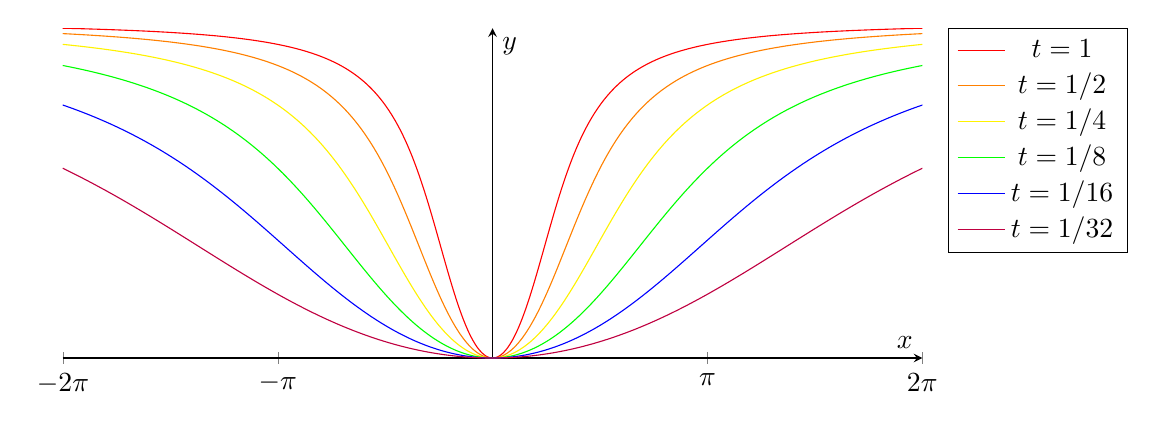
\begin{tikzpicture}
    \begin{axis}[
        xlabel=$x$,
        ylabel=$y$,
        width=12.5cm,
        height=5.77cm,
        xmin=-2*pi, xmax=2*pi,
        xtick={-6.28, -3.14, 0, 3.14, 6.28},
        xticklabels={$-2\pi$, $-\pi$, $0$, $\pi$, $2\pi$},
        ytick=\empty,
        axis lines=middle,
        samples=200,
        smooth,
        domain=-2*pi:2*pi,
        legend pos=outer north east,
    ]
    \addplot[red] {atan(x^2)};
    \addlegendentry{$t=1$}
    
    \addplot[orange] {atan(1/2*x^2)};
    \addlegendentry{$t=1/2$}
    
    \addplot[yellow] {atan(1/4*x^2)};
    \addlegendentry{$t=1/4$}
    
    \addplot[green] {atan(1/8*x^2)};
    \addlegendentry{$t=1/8$}
    
    \addplot[blue] {atan(1/16*x^2)};
    \addlegendentry{$t=1/16$}

    \addplot[purple] {atan(1/32*x^2)};
    \addlegendentry{$t=1/32$}
    \end{axis}
\end{tikzpicture}